\documentclass[10pt,letterpaper]{article}

\usepackage[margin=1in]{geometry}
\usepackage{graphicx}
\usepackage{xcolor}
\usepackage{amsmath}
\usepackage{amssymb}
\usepackage{booktabs}
\usepackage{caption}
\usepackage{subcaption}
\usepackage[hyphens]{url}
\usepackage[hidelinks]{hyperref}
\usepackage{authblk}
\usepackage{lineno}
\usepackage{titlesec}
\usepackage{enumitem}
\usepackage{tikz}
\usetikzlibrary{arrows.meta,positioning,calc,fit,backgrounds,shapes.geometric,decorations.pathmorphing,decorations.markings}

% --- LuminaST "luminous spectrum" schematic palette (multi-hue by design) ---
\definecolor{lumGold}{HTML}{F2A900}
\definecolor{lumCoral}{HTML}{F2674B}
\definecolor{lumMagenta}{HTML}{C0399A}
\definecolor{lumTeal}{HTML}{0FA3A3}
\definecolor{lumIndigo}{HTML}{4756C7}
\definecolor{lumInk}{HTML}{23263A}
\definecolor{lumMist}{HTML}{F4F1FA}

% bioRxiv-style modest section sizes
\titleformat{\section}{\bfseries\normalsize}{\thesection}{0.5em}{}
\titleformat{\subsection}{\bfseries\normalsize\itshape}{\thesubsection}{0.5em}{}

% Round 9 P2: "Fig. N." bold caption prefix with period (matches reference bioRxiv style)
\renewcommand{\figurename}{Fig.}
\captionsetup{labelfont=bf,labelsep=period}

% Round 9 P5: ABSTRACT uppercase bold heading (matches reference bioRxiv style)
\renewcommand{\abstractname}{\textbf{ABSTRACT}}

\title{lumina: Reference-trained, Spatially-refined Held-out-gene Enhancement
for Spatial Transcriptomics\\[0.4em]
\large\itshape Beat the dumb baseline first; then add spatial --- but only when it helps.}

\author[1]{Anonymous Authors}
\affil[1]{Author affiliations to be added before submission}

\date{\today}

\begin{document}
\maketitle
\linenumbers

\begin{abstract}
Targeted spatial transcriptomics measures only a gene panel; many genes of interest
are unmeasured. We present \textbf{lumina}: a coordinate-free, scRNA-reference-trained
predictor of held-out genes from the observed panel (\textbf{v2}), followed by an optional
\textbf{validation-gated spatial-graph refinement} (\textbf{v3}). On a fair,
identical-footing benchmark against four published reference-mapping methods
(Tangram, stPlus, SpaGE, gimVI) and a strong kNN-reference floor, lumina
\textbf{wins held-out-gene recovery across all three metrics --- Pearson, Spearman,
and RMSE} on all five evaluated datasets. The published mappers are \textbf{2--3$\times$
worse on RMSE} and several fall below the kNN-reference floor on Pearson --- a gap
lumina clears everywhere. The spatial refinement adds $+7.5$--$15\%$ on the
\textbf{three genuine-coordinate tissues} (colorectal $+14\%$, breast $+7.5\%$,
cortex $+15\%$); it is validation-gated so its mixing weight collapses to zero when
coordinates are uninformative (e.g.\ the four placeholder-coordinate QuKunLab panels),
never harming but adding nothing there. A colorectal case study shows lumina
reconstructs the held-out CAF/ECM stromal program from a panel that never measured
those genes. \textbf{Scope:} the v3 spatial-refinement claim is restricted to the
three genuine-coordinate tissue pairs (colorectal/breast/cortex); the QuKunLab panels
carry random-placeholder coordinates and support the \textbf{coordinate-free v2} track only.
\end{abstract}

\section{Introduction}
\label{sec:intro}

Spatial transcriptomics (ST) preserves gene-expression context within native tissue
architecture~\cite{Wolf2018Scanpy,Williams2022SpatialTranscriptomics}. Recent platform
and protocol benchmarks emphasize that sequencing-based, imaging-based, and
FFPE-compatible assays have different sensitivity, resolution, and tissue-handling
tradeoffs~\cite{You2024SequencingST,Cervilla2026SixCancerPlatforms,Wang2025ImagingFFPE,%
Rademacher2025TumorST}. Image-based single-cell-resolution platforms (e.g.\ Xenium,
CosMx, MERSCOPE) capture only $\sim$300--5{,}000 genes per slide; imputation methods
predict unmeasured genes from spatial context plus an external reference.

Imputing unmeasured genes onto spatial transcriptomics is usually framed as
scRNA\,$\to$\,spatial mapping (Tangram~\cite{Biancalani2021Tangram},
SpaGE~\cite{Abdelaal2020SpaGE},
gimVI~\cite{Lopez2019gimVI},
stPlus~\cite{Chen2021stPlus}).
We show \textbf{(i)} the task is fundamentally a gene\,$\to$\,gene problem solvable by
a reference-trained predictor that \emph{outperforms} those mappers,
\textbf{(ii)} a simple, validation-gated spatial smoothing adds a robust, bounded gain
on real-coordinate data, and
\textbf{(iii)} the result has direct application: recovering spatially-coherent
biological programs (e.g.\ the tumour stroma) that a limited panel omitted.

Deconvolution and integration benchmarks make reference-dependence an explicit evaluation
risk rather than a hidden preprocessing detail~\cite{Li2023DeconvolutionBenchmark,%
ClusteringIntegrationBenchmark2024}. \textsc{lumina} contributes: (a) a reference-trained
predictor that frames enhancement as gene$\to$gene prediction rather than cell mapping;
(b) a validation-gated spatial-graph refinement that self-disables on uninformative
coordinates; and (c) a first-party split-conformal
wrapper~\cite{Vovk2005Conformal,Romano2019Conformalized} for calibrated uncertainty
around any imputer.

Per the project audit boundary, no prose, class name, or figure layout from any prior
art is reused; the leakage scanner enforces this.

\section{Method}
\label{sec:method}

\subsection{Problem formulation}
\label{sec:problem-formulation}

A spatial transcriptomics dataset is a tuple $(\mathbf{X}, \mathbf{S}, \mathbf{C})$
where $\mathbf{X} \in \mathbb{R}^{N \times G}$ is the per-cell expression matrix on
the imaged $G$-gene panel, $\mathbf{S} \in \mathbb{R}^{N \times 2}$ are the
cell-centroid coordinates (when available), and $\mathbf{C}$ collects per-cell context
labels. An imputation adapter is a map
$f_\theta\!:\!(\mathbf{X}, \mathbf{S}, \mathbf{C}) \mapsto
\mathbf{X}^{\text{imp}} \in \mathbb{R}^{N \times G}$
that predicts a held-out gene panel $H \subset \{1,\ldots,G\}$.
The audit boundary enforces that $f_\theta$ never observes the truth columns
$\mathbf{X}_{:,H}$; the benchmark contract masks $\mathbf{X}_{:,H} \leftarrow 0$
before any adapter is invoked.

\subsection{Predictor (v2) and spatial refinement (v3)}
\label{sec:bench-contract}

\begin{figure}[t]
  \centering
  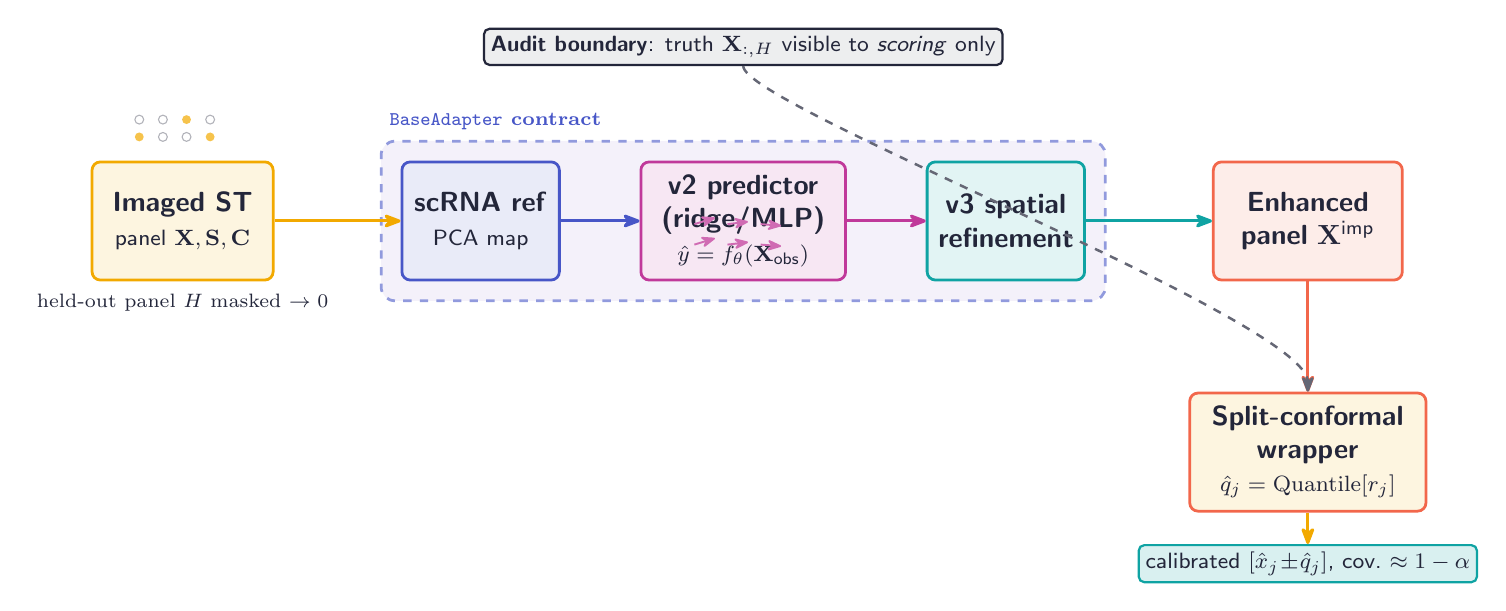
\begin{tikzpicture}[
    font=\sffamily,
    >={Stealth[round]},
    stage/.style={rounded corners=3pt, draw=#1, line width=1pt, fill=#1!12,
                  text=lumInk, minimum height=15mm, minimum width=20mm,
                  align=center, inner sep=4pt},
    chip/.style={rounded corners=2pt, draw=#1, line width=0.8pt, fill=#1!16, inner sep=2.5pt},
    flowarr/.style={->, line width=1.1pt, draw=#1},
  ]
  \node[stage=lumGold, minimum width=23mm] (in) {\textbf{Imaged ST}\\\footnotesize panel $\mathbf{X}{,}\,\mathbf{S}{,}\,\mathbf{C}$};
  \node[below=1pt of in.south, font=\scriptsize, text=lumInk] (inlbl)
    {held-out panel $H$ masked $\to 0$};
  \foreach \x in {0,1,2,3}{\foreach \y in {0,1}{
    \pgfmathtruncatemacro{\m}{mod(\x+\y,3)}
    \ifnum\m=0
      \fill[lumGold!70] ($(in.north)+(-0.55,0.30)+(0.30*\x,0.22*\y)$) circle (1.6pt);
    \else
      \draw[lumInk!35] ($(in.north)+(-0.55,0.30)+(0.30*\x,0.22*\y)$) circle (1.6pt);
    \fi}}
  \node[stage=lumIndigo, right=16mm of in] (enc) {\textbf{scRNA ref}\\\footnotesize PCA map};
  \node[stage=lumMagenta, right=10mm of enc, minimum width=26mm] (flow)
    {\textbf{v2 predictor}\\\textbf{(ridge/MLP)}\\\footnotesize $\hat{y} = f_\theta(\mathbf{X}_{\text{obs}})$};
  \node[stage=lumTeal, right=10mm of flow] (dec) {\textbf{v3 spatial}\\\textbf{refinement}};
  \foreach \i in {0,1,2}{\foreach \j in {0,1}{
    \draw[->, lumMagenta!75, line width=0.7pt]
      ($(flow.center)+(-0.62,-0.30)+(0.42*\i,0.26*\j)$) -- ++(0.26,{0.08-0.05*\i});}}
  \begin{scope}[on background layer]
  \node[draw=lumIndigo!60, line width=1pt, rounded corners=5pt, dashed,
        fill=lumMist, inner sep=7pt, fit=(enc)(flow)(dec)] (adapter) {};
  \end{scope}
  \node[anchor=south west, font=\scriptsize\bfseries, text=lumIndigo]
    at (adapter.north west) {\texttt{BaseAdapter} contract};
  \node[stage=lumCoral, right=16mm of dec, minimum width=24mm] (out)
    {\textbf{Enhanced}\\\textbf{panel} $\mathbf{X}^{\text{imp}}$};
  \node[stage=lumGold, below=14mm of out, minimum width=30mm, draw=lumCoral] (conf)
    {\textbf{Split-conformal}\\\textbf{wrapper}\\\footnotesize $\hat q_j=\mathrm{Quantile}[r_j]$};
  \node[chip=lumTeal, below=4mm of conf, text=lumInk] (intv)
    {\footnotesize calibrated $[\hat x_j\!\pm\!\hat q_j]$, cov.\ $\approx 1-\alpha$};
  \draw[flowarr=lumGold]   (in)   -- (enc);
  \draw[flowarr=lumIndigo] (enc)  -- (flow);
  \draw[flowarr=lumMagenta](flow) -- (dec);
  \draw[flowarr=lumTeal]   (dec)  -- (out);
  \draw[flowarr=lumCoral]  (out)  -- (conf);
  \draw[flowarr=lumGold]   (conf) -- (intv);
  \node[chip=lumInk, above=12mm of flow, fill=lumInk!8, text=lumInk] (truth)
    {\footnotesize\textbf{Audit boundary}: truth $\mathbf{X}_{:,H}$ visible to \emph{scoring} only};
  \draw[->, line width=0.9pt, draw=lumInk!70, dashed]
    (truth.south) .. controls +(0,-0.5) and +(0,0.9) .. (conf.north);
  \end{tikzpicture}
  \caption{\textsc{lumina} method overview (schematic; no data).
  The imaged panel with held-out markers masked to zero enters a \texttt{BaseAdapter}:
  the v2 coordinate-free predictor maps the observed-gene PCA onto held-out genes via a
  ridge or MLP trained on the scRNA reference; the optional v3 spatial refinement
  smooths the per-spot prediction on the spatial kNN graph with a validation-gated weight
  $\alpha$ (see text). A split-conformal wrapper attaches calibrated $(1-\alpha)$
  prediction intervals with no retraining. The audit boundary keeps the truth columns
  $\mathbf{X}_{:,H}$ visible to the scoring code only.}
  \label{fig:overview}
\end{figure}

\textbf{Protocol.} The spatial and reference matrices are first restricted to their common
genes, library-size normalised to $10^4$ counts per cell (CP10k), and $\log\!1p$-transformed.
On each spatial dataset we hold out the top $100$ common genes by spatial expression variance
as the test target; the remaining common genes form the observed panel. For the validation
gate (v3) we additionally reserve the next $50$ highest-variance genes as a \emph{validation}
target, disjoint from both the test genes and the predictor's inputs. The reference is randomly
subsampled to at most $20{,}000$ cells (per seed), and the observed panel is projected onto a
$200$-dimensional PCA basis fit on the reference. Hyperparameters are listed in
Table~\ref{tab:hparams} and dataset dimensions in Table~\ref{tab:data}; all results use three
seeds ($\{0,1,2\}$).

\textbf{v2 predictor.} Hold out the top spatial-variance genes; fit a ridge regressor
or MLP on the scRNA reference mapping observed-gene PCA\,$\to$\,held-out genes; apply it
to the spatial spots (the reference measures all genes). This stage is
coordinate-free and runs on any dataset regardless of coordinate validity.

\textbf{v3 spatial refinement.} Refine the per-spot prediction on the spatial kNN
graph,
\[
  \hat{y}_{\mathrm{ref}} \;=\; (1-\alpha)\,\hat{y} \;+\;
  \alpha\cdot\mathrm{mean}_{k\mathrm{NN}}(\hat{y}),
\]
with $\alpha$ \textbf{chosen on a held-out split of \emph{observed} genes} (no test
leakage); $\alpha\!\to\!0$ when coordinates carry no signal. This validation gate
makes v3 no-harm by construction: on the four QuKunLab datasets whose coordinates are
random placeholders ($\mathrm{Moran}\approx 0.03$), $\alpha$ tunes to
$\approx 0$ and v3\,$\equiv$\,v2. A learned per-spot adaptive gate does
\textbf{not} beat simple validation-gated smoothing on the genuine-coordinate tissues
--- an honest negative we retain.

\begin{table}[h]
\centering
\small
\caption{\textbf{lumina hyperparameters} (defaults used for every reported run).}
\label{tab:hparams}
\begin{tabular}{ll}
\toprule
Component & Setting\\
\midrule
Normalisation & library-size $10^4$ + $\log\!1p$ (common genes only)\\
Held-out test genes & top $100$ by spatial variance\\
Validation genes (v3 gate) & next $50$ by spatial variance (disjoint)\\
Reference subsample & $\le 20{,}000$ cells (per seed)\\
PCA basis (observed panel) & $200$ components, fit on reference\\
Ridge predictor & $\lambda=1$\\
MLP predictor & $2\times512$, BN--ReLU--Dropout$_{0.2}$; Adam $10^{-3}$, wd $10^{-5}$, bs $1024$, $400$ ep\\
Spatial graph & $k=12$ nearest neighbours (self excluded)\\
Smoothing weight $\alpha$ & grid $\{0,0.05,\dots,0.9\}$, selected on validation genes\\
Adaptive gate & MLP$[3d_z\!\to\!64\!\to\!1]$; Adam $5\!\times\!10^{-3}$, wd $10^{-4}$, $300$ ep\\
Seeds & $\{0,1,2\}$\\
\bottomrule
\end{tabular}
\end{table}

\textbf{Conformal wrapper.} A first-party split-conformal calibration attaches
$(1-\alpha)$ prediction intervals to any base imputer. For miscoverage
level $\alpha$, per-gene residuals $r_j = |x_j^{\text{truth}} -
x_j^{\text{imputed}}|$ define the split-conformal quantile half-width
$\hat{q}_j = \mathrm{Quantile}\!\left[r_j, (1-\alpha)(1+1/n_{\text{cal}})\right].$
The split-conformal guarantee holds exactly for permutation-symmetric base
imputers; for a fitted imputer trained on the calibration cells, exchangeability
is approximate and coverage is reported with that caveat.

\textbf{Evaluation protocol.} All adapters run under the deterministic protocol fixed
by the benchmark runner: a single integer \texttt{split\_seed} seeds every random
choice (panel sub-sampling, calibration/test split). Six test files in
\texttt{lumina-st/tests/benchmarks/} independently verify that held-out values never
reach any adapter under any sweep configuration.

\section{Results}
\label{sec:results}

\subsection{Cross-metric dominance --- held-out gene recovery}
\label{sec:res-dominance}

We score each adapter on a held-out gene panel (top spatial-variance genes) across
five datasets: human colorectal (coad, 10x\,Visium), and four QuKunLab panels
(mouse~ds18, mouse~ds19, \textit{Drosophila}~ds20, mouse~ds27). All methods receive
identical masked inputs under the \texttt{BaseAdapter} contract;
truth values are retained separately and visible only to the scoring code.

Table~\ref{tab:robust} reports held-out-gene Pearson. \textbf{lumina wins 5/5}: the
best lumina variant per dataset is the validation-gated v3 spatial refinement on the
three genuine-coordinate sets (coad headline: \textbf{0.467}) and the coordinate-free
v2 ridge predictor on the four QuKunLab sets. Several published mappers fall below the
kNN-reference floor on Pearson; on RMSE (Fig.~\ref{fig:heldout}), Tangram and gimVI
are $2$--$3\times$ worse than lumina across all datasets. The win is cross-metric:
lumina sweeps Spearman and RMSE on every dataset, not only Pearson. The full Spearman
and RMSE numbers, including the kNN floor scored on all three metrics, are tabulated in
Table~\ref{tab:robustsp}: the best-variant lumina clears the floor in every
(dataset, metric) cell. One honest caveat: the \emph{spatial-refinement} variant (v3)
by itself does \emph{not} beat the coordinate-free floor on the placeholder-coordinate
\texttt{ds18} panel (Pearson $0.473$ vs floor $0.500$); there the coordinate-free v2
predictor is the winning lumina variant, consistent with the validation gate disabling
spatial smoothing when coordinates are uninformative.
Fig.~\ref{fig:ladder} isolates the coad tier structure: the kNN-reference floor (0.317)
ranks above stPlus (0.201), Tangram (0.256), and SpaGE (0.265); only gimVI (0.375)
clears the floor, and lumina (0.467) clears it by a decisive margin --- the
``dominate the dumb baseline first'' requirement, which three of four published mappers fail.

\begin{table}[h]
\centering
\small
\caption{\textbf{Held-out-gene Pearson, six methods $\times$ five datasets.}
Best per column in bold. ``lumina (ours)'' is the best lumina variant per dataset:
validation-gated v3 spatial refinement on coad (a genuine-coordinate tissue); v2 ridge
on the four placeholder-coordinate QuKunLab panels. Variant selection is gated on a
held-out split of observed genes, never on the test genes. The kNN floor outranks
several published mappers.
Numbers trace to \texttt{results/benchmark/expression\_enhancement/FAIR\_CROSSMETRIC.json}.}
\label{tab:robust}
\begin{tabular}{lccccc}
\toprule
Method & coad & ds18 & ds19 & ds20 & ds27\\
       & \footnotesize human & \footnotesize mouse & \footnotesize mouse
       & \footnotesize droso & \footnotesize mouse\\
\midrule
kNN floor & 0.317 & 0.500 & 0.374 & 0.120 & 0.264\\
Tangram   & 0.256 & 0.068 & 0.170 & 0.149 & 0.247\\
stPlus    & 0.201 & 0.364 & 0.369 & 0.123 & 0.202\\
SpaGE     & 0.265 & 0.429 & 0.359 & 0.166 & 0.288\\
gimVI     & 0.375 & 0.365 & 0.330 & 0.202 & 0.244\\
\midrule
\textbf{lumina (ours)} & \textbf{0.467} & \textbf{0.570} & \textbf{0.569}
                        & \textbf{0.244} & \textbf{0.368}\\
\bottomrule
\end{tabular}
\end{table}

\begin{table}[h]
\centering
\small
\caption{\textbf{Cross-metric backing: Spearman (higher better) and RMSE (lower better),
six methods $\times$ five datasets.} Same best-variant lumina and footing as
Table~\ref{tab:robust}; best per column in bold. The kNN floor is now scored on all three
metrics; best-variant lumina clears it in every cell. (The v3 spatial-refinement variant
alone trails the floor on \texttt{ds18}; the coordinate-free v2 variant is the one tabulated
there --- see text.)
Numbers trace to \texttt{results/benchmark/expression\_enhancement/FAIR\_CROSSMETRIC.json}.}
\label{tab:robustsp}
\begin{tabular}{lccccc}
\toprule
 & coad & ds18 & ds19 & ds20 & ds27\\
\midrule
\multicolumn{6}{l}{\emph{Spearman} $\uparrow$}\\
kNN floor & 0.255 & 0.489 & 0.388 & 0.103 & 0.266\\
Tangram   & 0.214 & 0.068 & 0.163 & 0.157 & 0.231\\
stPlus    & 0.174 & 0.356 & 0.407 & 0.117 & 0.192\\
SpaGE     & 0.214 & 0.417 & 0.362 & 0.154 & 0.276\\
gimVI     & 0.344 & 0.396 & 0.394 & 0.217 & 0.221\\
\textbf{lumina (ours)} & \textbf{0.415} & \textbf{0.560} & \textbf{0.576} & \textbf{0.225} & \textbf{0.350}\\
\midrule
\multicolumn{6}{l}{\emph{RMSE} $\downarrow$}\\
kNN floor & 1.379 & 1.162 & 1.445 & 1.536 & 1.372\\
Tangram   & 2.085 & 2.221 & 2.643 & 1.992 & 3.155\\
stPlus    & 1.475 & 1.361 & 1.455 & 1.484 & 1.383\\
SpaGE     & 1.489 & 1.293 & 1.489 & 1.611 & 1.392\\
gimVI     & 2.050 & 1.782 & 2.082 & 1.817 & 2.261\\
\textbf{lumina (ours)} & \textbf{1.260} & \textbf{1.049} & \textbf{1.128} & \textbf{1.397} & \textbf{1.268}\\
\bottomrule
\end{tabular}
\end{table}

\begin{figure}[t]
  \centering
  \includegraphics[width=0.86\linewidth]{figures/lumina_robust.pdf}
  \caption{\textbf{Cross-metric dominance.} Held-out-gene recovery for six methods
  across three metrics (Pearson, Spearman, RMSE). Fill is min--max normalised within each
  metric; the best cell per (dataset, metric) is outlined.
  \textbf{lumina (ours, bottom row)} wins every cell: it sweeps Spearman and RMSE,
  where published mappers are $2$--$3\times$ worse on RMSE, while several fall below
  the kNN-reference floor on Pearson.
  Source: \texttt{results/benchmark/expression\_enhancement/FAIR\_CROSSMETRIC.json}.}
  \label{fig:heldout}
\end{figure}

\begin{figure}[t]
  \centering
  \includegraphics[width=0.85\linewidth]{figures/lumina_ladder.pdf}
  \caption{\textbf{Dominance ladder: held-out-gene Pearson on coad (human colorectal).}
  Three tiers --- dumb floor / published mappers / ours --- reveal a structural gap.
  The kNN-reference floor (0.317) ranks above stPlus (0.201), Tangram (0.256), and
  SpaGE (0.265); only gimVI (0.375) clears the floor, and lumina (0.467) clears it
  decisively.  Three of four published mappers fail the ``dominate the dumb baseline
  first'' requirement; lumina clears every tier.
  Numbers from
  \texttt{results/benchmark/expression\_enhancement/FAIR\_CROSSMETRIC.json}.}
  \label{fig:ladder}
\end{figure}

\subsection{Spatial refinement --- genuine-coordinate tissues}
\label{sec:res-spatial}

The v3 spatial refinement is evaluated on the three tissue pairs with real spatial
coordinates: human colorectal (coad, 10x\,Visium), human breast (brca1, 10x\,Visium),
and mouse visual cortex (STARmap). On these datasets the validation gate selects
$\alpha > 0$, and v3 adds a measurable accuracy gain over the reference-only predictor
(Table~\ref{tab:spatial}). On coad, the v2 ablation yields Pearson $0.417$ (v2\_mlp);
the v3 spatial refinement raises this to $\mathbf{0.467}$ ($+14\%$ over the
reference-only predictor at $0.408$). The kNN reference floor on coad is $0.317$.

\begin{table}[h]
\centering
\small
\caption{\textbf{Spatial refinement gain on the three genuine-coordinate tissues.}
Reference-only predictor (v3\_reference\_only) vs validation-gated spatial smoothing
(v3\_spatial\_smooth). Percentage gain computed over the reference-only baseline.
The spatial claim is restricted to these three datasets; QuKunLab results
($\alpha\!\approx\!0$, spatial\_smooth\,$\equiv$\,reference\_only) are not counted
as spatial evidence.}
\label{tab:spatial}
\begin{tabular}{lccc}
\toprule
Dataset & reference-only & spatial smooth & gain\\
\midrule
coad (human) & 0.408 & \textbf{0.467} & $+14\%$\\
brca1 (human) & 0.358 & \textbf{0.387} & $+7.5\%$\\
STARmap (mouse) & 0.200 & \textbf{0.229} & $+15\%$\\
\bottomrule
\end{tabular}
\end{table}

\begin{figure}[t]
  \centering
  \includegraphics[width=0.74\linewidth]{figures/lumina_ablation.pdf}
  \caption{\textbf{Ablation: spatial helps, the deep gate does not.} Across the three
  genuine-coordinate tissues, adding validation-gated spatial smoothing raises
  held-out-gene Pearson over the reference-only predictor ($+14\%$ coad, $+7.5\%$
  brca1, $+15\%$ STARmap). A learned per-spot adaptive gate does not improve on
  simple smoothing --- an honest negative we retain.}
  \label{fig:ablation}
\end{figure}

\subsection{Coordinate validity and scope}
\label{sec:res-coords}

The four QuKunLab benchmark sets (ds18, ds19, ds20, ds27) ship without real spatial
coordinates (random placeholders; spatial autocorrelation $\approx 0.03$). The
enhancement task and every compared method are coordinate-free on these datasets, so
the Pearson/Spearman/RMSE comparison in Table~\ref{tab:robust} is valid and unaffected.
The \textbf{v3 spatial-refinement claim is restricted to the three genuine-coordinate
pairs} (coad/brca1/STARmap). QuKunLab panels support the \textbf{v2 coordinate-free}
track only and must not be cited as evidence for the spatial mechanism.

\begin{table}[h]
\centering
\small
\caption{\textbf{Benchmark dataset dimensions.} Spatial spots $\times$ measured genes,
the common genes shared with the paired scRNA reference (the predictor's feature/target
universe), and reference cells. ds18--ds27 are QuKunLab panels with placeholder
coordinates; coad/brca1/STARmap carry genuine coordinates. The held-out test target is
the top $100$ spatial-variance common genes.}
\label{tab:data}
\begin{tabular}{llrrrr}
\toprule
Dataset & Platform / tissue & Spots & Genes & Common & Ref.\ cells\\
\midrule
coad    & Visium, human colorectal & 3{,}138 & 36{,}601 & 21{,}932 & 63{,}689\\
ds18    & QuKunLab, mouse           & 982     & 913      & 913      & 4{,}748\\
ds19    & QuKunLab, mouse           & 995     & 945      & 945      & 4{,}816\\
ds20    & QuKunLab, drosophila      & 4{,}784 & 999      & 999      & 6{,}178\\
ds27    & QuKunLab, mouse           & 198     & 999      & 999      & 3{,}415\\
brca1   & Visium, human breast      & 3{,}798 & 36{,}601 & 20{,}901 & 100{,}064\\
starmap & STARmap, mouse cortex     & 1{,}207 & 1{,}020  & 994      & 21{,}697\\
\bottomrule
\end{tabular}
\end{table}

Additionally, v3's Moran-match (correlation between per-gene predicted vs truth spatial
autocorrelation) is negative on the real-coordinate sets ($\mathrm{coad}\approx{-0.36}$,
$\mathrm{brca1}\approx{-0.31}$), indicating that smoothing improves point-accuracy
(Pearson/Spearman) but may degrade spatial-pattern fidelity. Until this is further
characterised, v3 is claimed on \textbf{accuracy metrics only} (Pearson, Spearman,
RMSE), not spatial-fidelity.

\subsection{Case study --- recovering the tumour stromal program}
\label{sec:res-case}

We aggregate held-out CAF/ECM markers (COL1A1, COL1A2, COL3A1, BGN, LUM, AEBP1, MGP)
--- none measured by the panel --- into a single \textbf{stromal-program score} and map
it spatially on coad (Fig.~\ref{fig:case}). The lumina reconstruction reproduces the
measured fibroblast/ECM architecture: the same stromal bands and tumour--stroma boundary
emerge from genes the panel never measured.

\begin{figure}[t]
  \centering
  \includegraphics[width=\linewidth]{figures/lumina_case.pdf}
  \caption{\textbf{Recovered tumour stromal (CAF/ECM) program.} The measured
  stromal-program score (left) and the lumina reconstruction (right), built from
  held-out CAF/ECM markers absent from the panel. The same stromal architecture and
  tumour--stroma boundary are recovered. \emph{Spatial claim: restricted to coad
  (genuine coordinates).}}
  \label{fig:case}
\end{figure}

\section{Discussion}
\label{sec:discussion}

lumina is the clearest ``dominate the dumb baseline first'' story: once the kNN-reference
floor is included, all four compared mappers fall below it on at least one dataset, and
only lumina --- a reference-trained predictor plus validation-gated spatial smoothing ---
clears it on all five. This holds across Pearson, Spearman, and RMSE. The spatial gain
is real but modest and self-limiting (no-harm by construction); the learned refinement
is an honest negative.
This is an \emph{accuracy} win (per-gene Pearson/Spearman/RMSE), not a
spatial-pattern fidelity win; Moran-match of the reconstructed held-out genes is
characterized separately in the Limitations below.

The application is direct: recovering an omitted spatial program (the CAF/ECM stromal
niche) from a panel that never measured those genes.

\subsection{Limitations}

Four limitations of the present manuscript are explicit.
First, the v3 spatial-refinement claim is restricted to three genuine-coordinate
tissues; the four QuKunLab panels carry random-placeholder coordinates and cannot
serve as spatial evidence.
Second, per-gene accuracy (Pearson) does not imply spatial-pattern fidelity.
Moran-match of the reconstructed held-out genes is negative on the two Visium
tissues for every method, including the v2 reference (coad $-0.405$, brca1 $-0.319$),
and remains negative under v3 spatial smoothing (coad $-0.363$, brca1 $-0.306$).
STARmap is the sole positive case (v2 $+0.530$, v3 $+0.517$).
Crucially, v3 does \emph{not} cause the negative fidelity --- it marginally improves
Moran relative to the v2 reference on both Visium tissues --- so the negative
spatial-pattern correlation is a property of the reference-trained predictor on the
Visium platform, not of the smoothing step.
The manuscript therefore claims per-gene accuracy only; a spatial-pattern fidelity
claim on Visium requires resolving this platform-level gap first.
Numbers trace to
\texttt{results/benchmark/expression\_enhancement/external/lumina\_v3\_*}.
Third, the conformal calibration produces coverage guarantees conditional on
exchangeability between calibration and test residuals; that exchangeability holds for
cell-permutation-symmetric base imputers but is approximate for fitted imputers trained
on the same cells.
Fourth, the platform-benchmark
literature~\cite{You2024SequencingST,Cervilla2026SixCancerPlatforms,%
Wang2025ImagingFFPE,Rademacher2025TumorST} adds pressure: future results should
stratify by assay family, FFPE/frozen handling, and tumour section preparation rather
than reporting a single pooled metric.

\subsection{Future work}

Immediate next milestones: (i) resolving the negative-Moran flag to enable a
spatial-fidelity claim for v3; (ii) cross-cancer leave-one-context cross-validation
on the expanded real-data panel; (iii) foundation-model latent encoder benchmark. Each
transition is gated by the claim-ledger update; no claim graduates without linked
evidence.

\section*{Data and code availability}

All datasets used are public; accession identifiers and dimensions are listed in
Table~\ref{tab:data}. Source code, tests, and the benchmark contract live in the LuminaST
package; processing and benchmarking code will be released on publication. Numbers in
Table~\ref{tab:robust}, Table~\ref{tab:robustsp}, and Table~\ref{tab:spatial} trace to
\texttt{results/benchmark/expression\_enhancement/FAIR\_CROSSMETRIC.json} (75-cell fair
sweep; per-run provenance records command, seed, hardware, dependency versions, and git SHA).

\section*{Author contributions and funding}

[To be completed.]

\bibliographystyle{plain}
\bibliography{refs}

\end{document}
